\unnumberedchapter{Introduction}


\eg
In recent years, Machine Learning techniques have revolutionized solutions to longstanding image-based
problems, like image classification, generation, semantic segmentation, object detection and many others.
However, if we want to be able to build agents that can successfully interact with the real world,
those techniques need to be capable of reasoning about the world as it truly is: a tridimensional space.
There are two main challenges while handling 3D information in machine learning models.
First, 3D data is not available in the same scale as images -- taking pictures is a common procedure in
our daily lives, whereas capturing 3D content is an activity usually restricted to specialized
professionals.
Second, it is not clear what is the best 3D representation for machine learning models.
For images, convolutional neural networks (CNNs) operating on raster images yield the best results in
virtually all image-based benchmarks.
For 3D data, the best combination of model and representation is still an open question.
My research is focused in addressing both of these issues.
Which model and representation should we use for generating~\cite{pcagan, mrt} and recognizing~\cite{shapeclassifiers, mrt} 3D data?
Is it possible to leverage image data to build models capable of reasoning about the world in 3D~\cite{gadelha19deepshape, prgan, prganpp}?

Our research findings show that we are able to build models that efficiently generate 3D shapes as unstructured point clouds.
Those models require significantly less memory while generating higher quality shapes than the ones based
on voxels and multi-view representations.
% We start by demonstrating that one can leverage spatial-partitioning structures to assign an approximate
% correspondence between points of different point clouds.
% Using this correspondence, we compute a linear low-dimensional shape representation that can be used to
% train Generative Adversarial Networks (GANs) for point cloud generation.
% We then extend this model by computing non-linear shape representations using custom convolutional
% architectures trained end-to-end with permutation invariant losses.
These architectures can be applied to shape classification, segmentation, single-view reconstruction and
unsupervised representation learning with variational auto-encoders (VAEs).
Notwithstanding, the aforementioned techniques require explicit 3D supervision, which is scarce.
Ideally, we want to be able to use images as supervisory signal while learning to generate 3D data.
We tackle this problem by proposing differentiable neural network modules capable of generating images from 3D representations.
The experiments demonstrate that those modules can serve as building blocks to neural network architectures, enabling learning 3D representations from 2D images in a variety of scenarios.
% If there are multiple images of various objects without viewpoint annotations, the projection modules can
% be used to create a variation of GANs, which we call Projective GANs (PrGANs), capable of generating
% 3D shapes without ever receiving explicit 3D supervision, just images of object silhouettes.
% This problem is particularly challenging because we don't even have any object identification, i.e. we don't know which images correspond to the same object, rendering multi-view techniques unfeasible.
% Additionally, we demonstrate that convolutional architectures can induce priors over 3D shapes and by coupling them with projection modules we derive a class of powerful reconstruction techniques that
% does not rely on task-specific training.
% We also design new differentiable projection modules that enable learning 3D shapes from depth maps and sinograms,
% yielding state-of-the-art results for tomographic reconstruction.

Below, I address the specific topics of my research in more detail.

\subsection*{Learning from Unstructured Data}

Tridimensional occupancy grids are a natural choice for representing 3D data in deep neural networks.
They are a straightforward extension to raster images and convolutional layers can be seamlessly
applied to this type of data.
Another way to represent 3D data is by simply utilizing multiple 2D images of a 3D object.
We refer to this as multi-view representation.
This type of representation can also be easily integrated with convolutional layers and even
offers the extra advantage of being able to leverage image features pre-trained from massive image
datasets.
As a matter of fact, we demonstrate in \cite{shapeclassifiers} that multi-view representations are still the
state-of-the-art for shape classification tasks.

\begin{figure}
 \begin{center}
 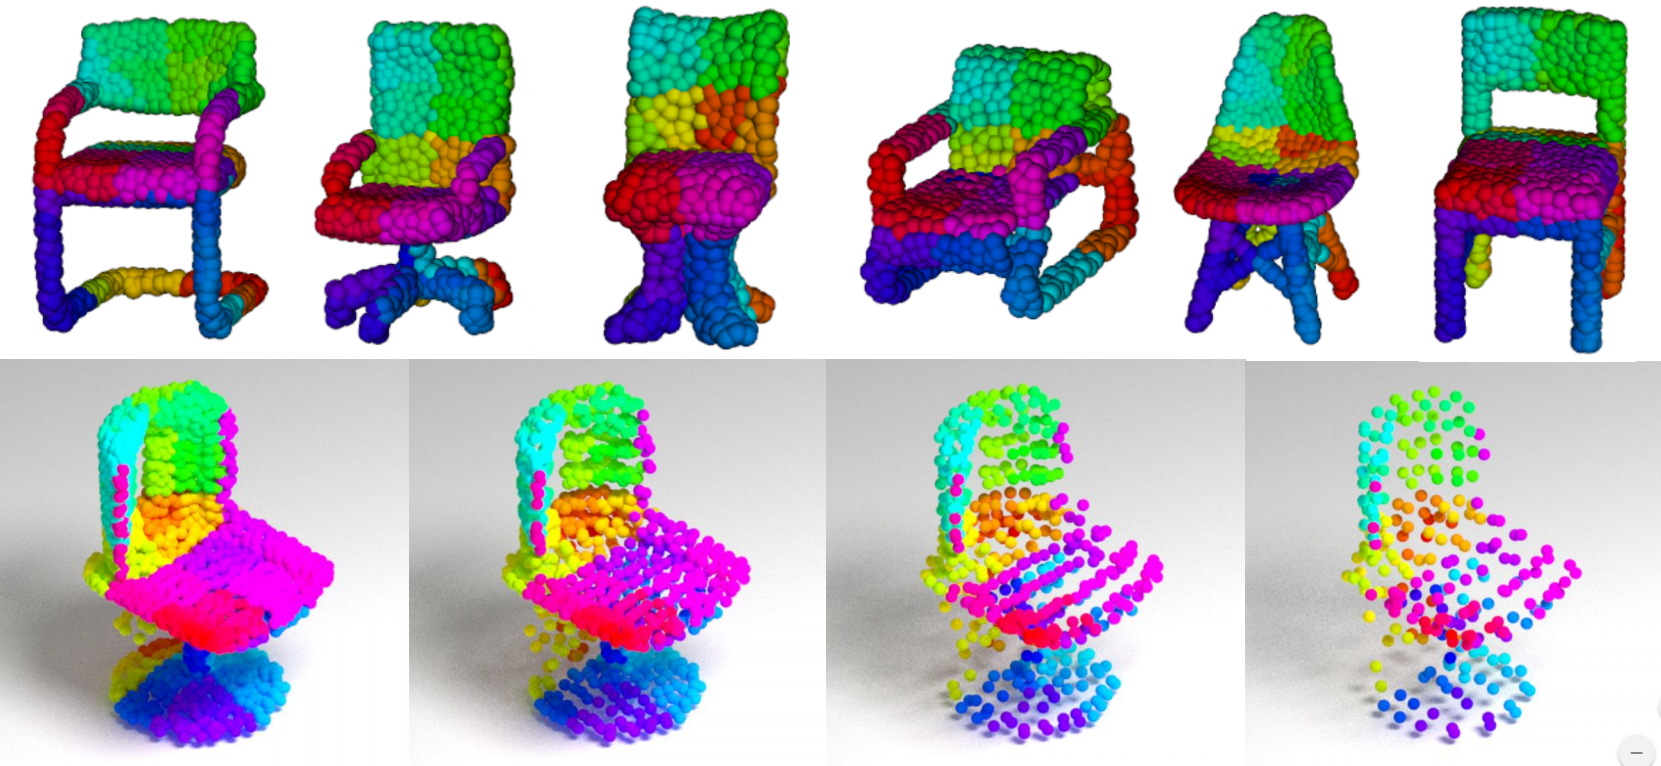
\includegraphics[width=\linewidth]{figs/shapepartition.png}
 \end{center}
 \vspace{-20pt}
 \caption{\small Point clouds sorted according to spatial partitioning structures induce
 reasonable point correspondence (indicated by similar colors).
 The same structure can also be used to compute multiple point cloud resolutions.
 We build upon these observations to design multi-resolution convolutional operators
 for point cloud data.}
\end{figure}

However, generating 3D shapes poses a more challenging situation.
While generating 3D data, we are primarily concerned about generating surfaces, which are
inherently sparse in the 3D space.
This leads to a big drawback for occupancy grids: models using them require huge amounts of memory,
being prohibitively large when generating high-resolution shapes.
For multi-view representations, there are two main issues:
first, these representations are restricted to representing only the visible portion of the surface --
interior parts are not represented.
Second, it is not clear how to enforce consistency between different views, which leads to a reduced quality in the generated shapes.
A way to workaround the later is to enforce consistency through a post-processing optimization step, like the one we developed in~\cite{sketch}.
Nevertheless, these models are still very memory intensive and do not handle generating
multiple categories of objects.

A reasonable alternative to those 3D representations is utilizing point clouds.
Point clouds are a very compact surface representation -- every point in the point must be part of the surface.
They also naturally support extra surface attributes, like color and normals, and are directly captured by a variety of 3D sensors.
The biggest challenge while using point clouds in deep networks lies in its unstructured nature.
Since they are sets of points, point cloud representations need to be invariant to permutations.
Moreover, differently form multi-view representations and occupancy grids, it is not clear what is the best way to use convolutional layers in point cloud data.

Our attempt in creating generative models for point clouds was bootstrapped by using spatial-partitioning data-structures to assign an approximate correspondence between points of
different point clouds~\cite{pcagan}.
The motivation is simple: if one can induce such correspondence, point clouds can be treated as structured data.
In practical terms, we compute a $kd$-tree for every point cloud and sort the points according to a level-order traversal in the leaves of the tree.
This sorting induces a reasonable correspondence between points, as shown in Figure 1.
Using this correspondence, we compute a linear low-dimensional shape representation that were used to
train the first Generative Adversarial Networks (GANs) for point cloud generation~\cite{pcagan}.
Later, we noticed that the spatial partitioning induces a local neighborhood that can be successfully
used to define convolutional operations and to represent multiple point cloud resolutions~\cite{mrt}.
\begin{figure}
\vspace{-20pt}
 \begin{center}
 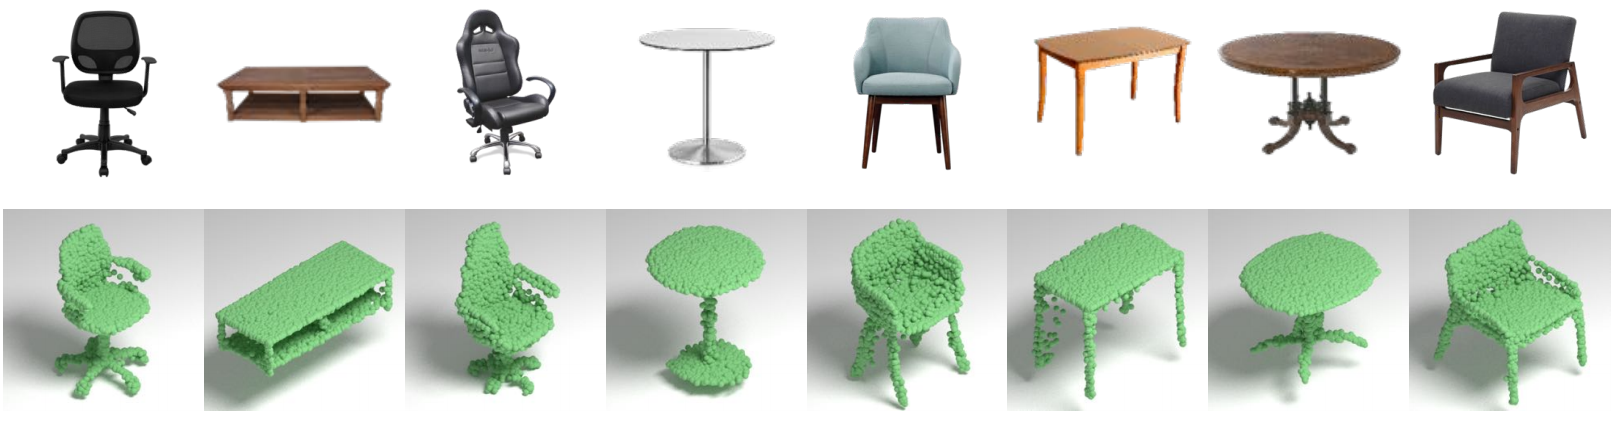
\includegraphics[width=\linewidth]{figs/mrtresults.png}
 \end{center}
 \vspace{-20pt}
 \caption{\small Single-view reconstruction using MRTNets.}
 \vspace{-5pt}
\end{figure}
We called these models Multi-Resolution Tree Networks (MRTNets) and applied them to a variety of
discriminative and generative tasks, like shape classification, 
part segmentation, single-view reconstruction and VAEs.
Some of the results are presented in Figure 2.
The models have a small memory footprint when compared against multi-view and occupancy grids counterparts while yielding state-of-the-art results for point cloud classification, single-view reconstruction and
unsupervised feature learning benchmarks.


\subsection*{Learning 3D Shapes from Images}

Images are much more prevalent than 3D data.
The most used shape classification benchmark, ModelNet40, contains about 10 thousand shapes,
whereas the most popular image classification benchmark, ImageNet, contains about 14 million images.
Nevertheless, images usually contain real world entities which are inherently 3D.
In other words, a lot of 3D information is encoded in images and being able to leverage that information
to learn to generate 3D shapes is key to build models that can overcome the lack of 3D training data.
We study this issue within a very challenging problem setup.
Consider a set of silhouette images like the ones in Figure 3.
Those images represent silhouettes of various objects from the same category.
If we have viewpoint annotation and object identification (i.e. which images correspond to the same object) this problem can be easily solved using visual hull.
We can make the problem harder by assuming that no viewpoint annotation is available.
In that case, we can probably achieve a reasonable result by relying in Structure from Motion (SfM) techniques.
The most difficult setup occurs when we neither have object identification nor viewpoint annotation.
In this scenario, one can only rely on non-rigid SfM, which require a strong prior over the generated shapes.
What happens when we have no information regarding 3D shapes? Can we still do something about it?


\begin{figure}
\vspace{-20pt}
 \begin{center}
 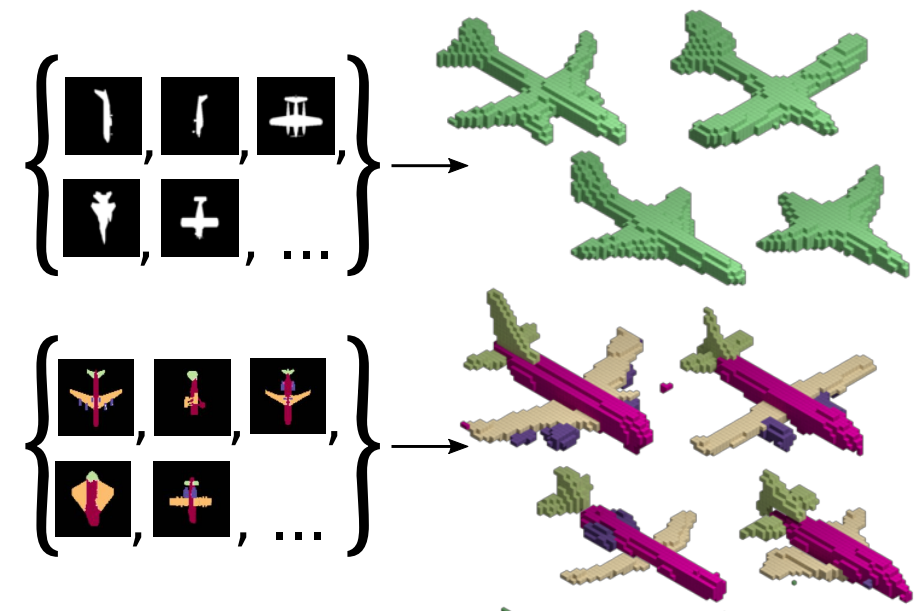
\includegraphics[width=\linewidth]{figs/prganpp.png}
 \end{center}
 \vspace{-20pt}
 \caption{\small PrGAN is capable of learning generative models of 3D data without using any 3D supervision.
 The core of the approach is the utilization of differentiable projection operators
 that turn 3D representation into images of silhouettes and segmentation masks.}
 \vspace{-5pt}
\end{figure}
Our solution consists of utilizing deep generative models coupled with differentiable projection operators.
The intuition is simple: given a dataset with images, we want to generate 3D shapes that, when projected into the image plane, will look like they came from the dataset.
More precisely, we want to match the distribution of images in the dataset to the images created by projecting the generated 3D shapes.
Fortunately, there is a class of deep learning models which is remarkably good in mimicing target image
distributions: generative adversarial networks (GANs).
Thus, we augment the GAN generator with a differentiable shape projection module which turns 3D shapes into silhouette images.
The result is a 3D generative model that is trained without ever seeing any 3D data, only silhouettes of 3D objects.
We name this model Projective GAN (PrGAN)~\cite{prgan}.
Later, we extended this architecture to enable learning from extra image annotations (e.g. part segmentation) by designing projection modules capable of generating part-segmented images~\cite{prganpp}.

Another interesting scenario occurs when we don't have access to images of multiple objects,
but only a small set images of a single object with viewpoint annotations.
In that case, visual hull techniques are applicable, but we can do better than that, even without
using any extra training data.
We build upon priors induced by deep image models~\cite{bayesiandip} and
demonstrate that convolutional architectures can also induce priors over 3D shapes.
We can then combine them with projection modules, deriving a class of powerful reconstruction techniques that
does not rely on task-specific training.
Additionally, by doing inference through descent we can update viewpoint estimations, enabling reconstruction with noisy viewpoint annotations.
We also design new differentiable projection modules that enable learning 3D shapes from depth maps and sinograms,
yielding state-of-the-art results for tomographic reconstruction~\cite{gadelha19deepshape} and visual hull.